\documentclass{llncs}

\usepackage{graphicx}
\usepackage{mwe}
\usepackage{subfig}
\usepackage{amsmath}
\usepackage{amssymb}
\usepackage{rotating}

\begin{document}

\title{Numerical modelling of quantum harmonic oscillator}
\author{Pawel Czyz}

\authorrunning{Pawel Czyz}

\institute{St Hugh's College, University of Oxford,\\
St Margaret's Road, Oxford OX2 6LE, UK}

\maketitle

\begin{abstract}
We present a Python module implementing various ODE solvers, enabling one to do accurate and effective numerical simulations. We investigate it's accuracy investigating a quantum harmonic oscillator in position basis.

\keywords{numerical modelling, Numerov's algorithm, quantum systems, harmonic oscillator}
\end{abstract}

\section{Introduction}
Numerov's method [1] allows one to solve differential equations of kind:

\begin{equation}
\label{eq:num}
	y''(x) = f(x)\cdot y(x)
\end{equation}

Examples of equation (\ref{eq:num}) include classical harmonic oscillator:

\begin{equation}
\label{eq:harm}
	y''(x) = -\omega^2\cdot y(x)
\end{equation}

or one-dimensional, time-independent Schrodinger's equation:
\begin{equation}
\label{eq:quant}
	y''(x)=\frac{2m}{\hbar^2}(E-V(x))\cdot y(x).
\end{equation}

Numerov's iterative metod uses an equidistant grid [1,2] $x_n=\delta n$ on which approximates $y_i$ values via equation:

\begin{equation}
\label{eq:iter}
	\left(1-\frac {\delta^2}{12}f_{n+2}\right)y_{n+2}=\left(2+\frac 56\delta^2 f_{n+1}\right)y_{n+1}-\left(1-\frac{\delta^2}{12}f_n\right)y_n,
\end{equation}

where $f_i=f(x_i)$. Equation (\ref{eq:iter}) can be solved for arbitrary $n$ knowing the values $y_0$ and $y_1$.

In practice, second-order differential equations are given Cauchy boundary conditions - $y(0)=y_0$ and $y'(0)=v_0$. Therefore, value $y_1$ is often approximated
using Taylor polynomial:
\begin{equation}
\label{eq:taylor}
y_1=y(\delta)\approx y(0)+ \sum_{n=1}^4 \frac{\delta^n}{n!} y^{(n)}(0).
\end{equation}

Differentiating equation (\ref{eq:num}) and substituting $y''$ for combinations of $y$ and $f$ one gets the fourth-order approximation in terms of $y_0$, $v_0$ and values of different derivatives of $f$, which can be evaluated symbolically or numerically:
\begin{align}
\label{eq:approx}
	y_1 \approx \frac{1}{24} \delta ^4\left(y_0 f''(0)+2 f'(0) v_0+f_0^2 y_0\right) + \\
	+\frac{1}{6} \delta ^3 \left(y_0 f'(0) +f_0 v_0\right)+\frac{1}{2} \delta ^2 f_0
   y_0+\delta  v_0+y_0
\end{align}

\section{Quantum harmonic oscillator}
Schrodinger equation for quadratic potential $V(x)\propto x^2$ can be written is dimensionless form as:
$$y''(x)$$ 
\section{Conclusions}

\begin{figure}
\centering
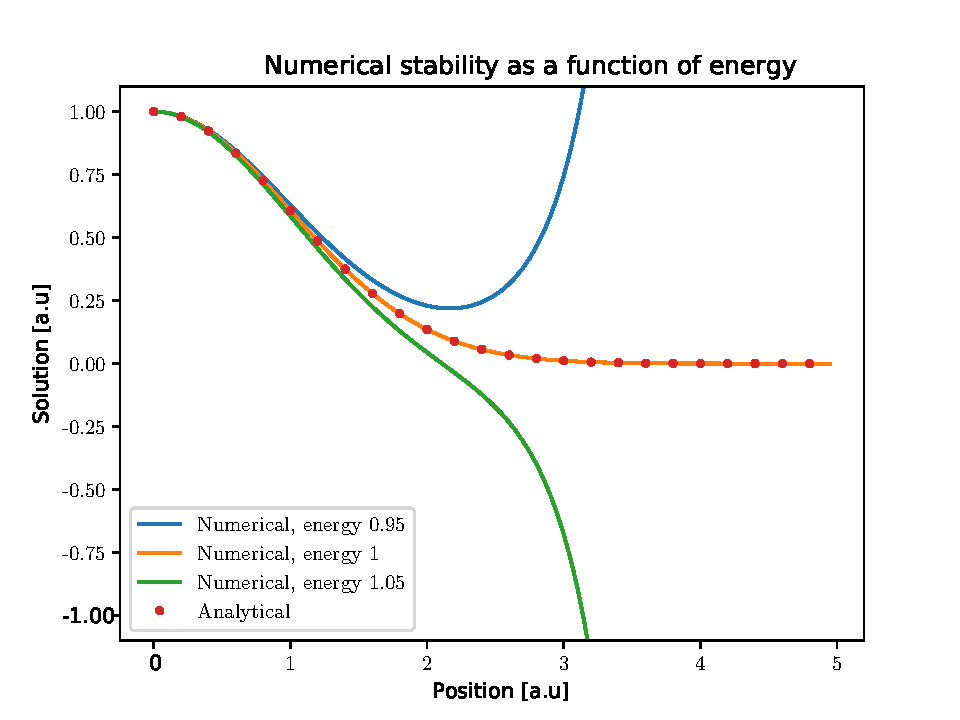
\includegraphics[width=0.7\textwidth]{images/Quantum_oscillator-0}
\caption{Mock - just a template how to insert images.}
\label{fig:mock}
\end{figure}

\begin{figure}
\centering
\begin{minipage}{.47\linewidth}
\centering
\subfloat[]{\label{fig:prec:a}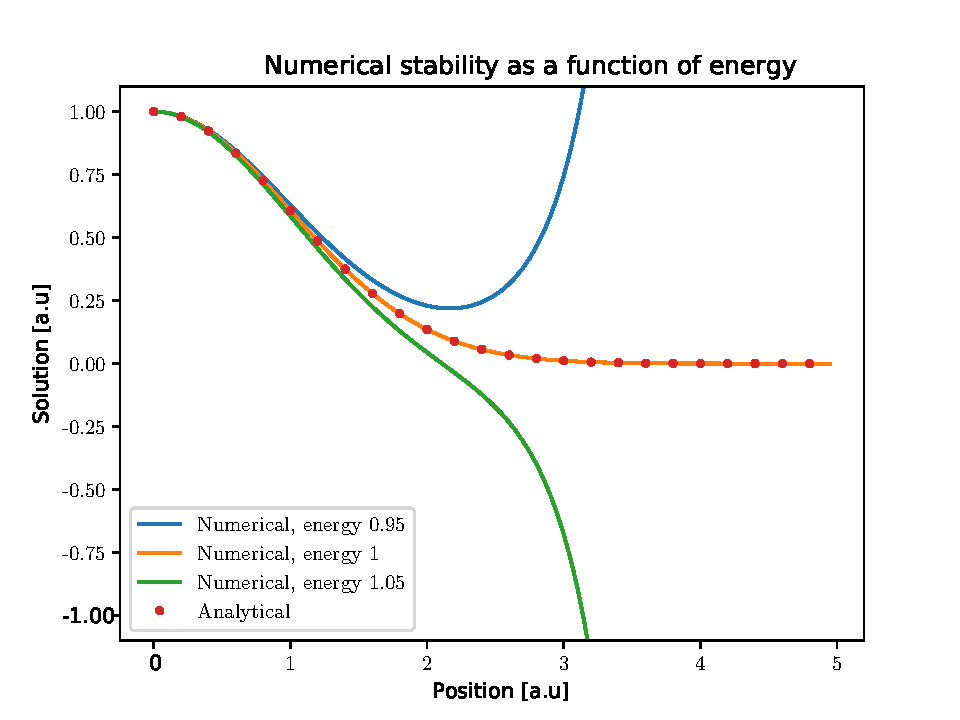
\includegraphics[width=\textwidth]{images/Quantum_oscillator-0}}
\end{minipage}
\begin{minipage}{.47\linewidth}
\centering
\subfloat[]{\label{fig:prec:b}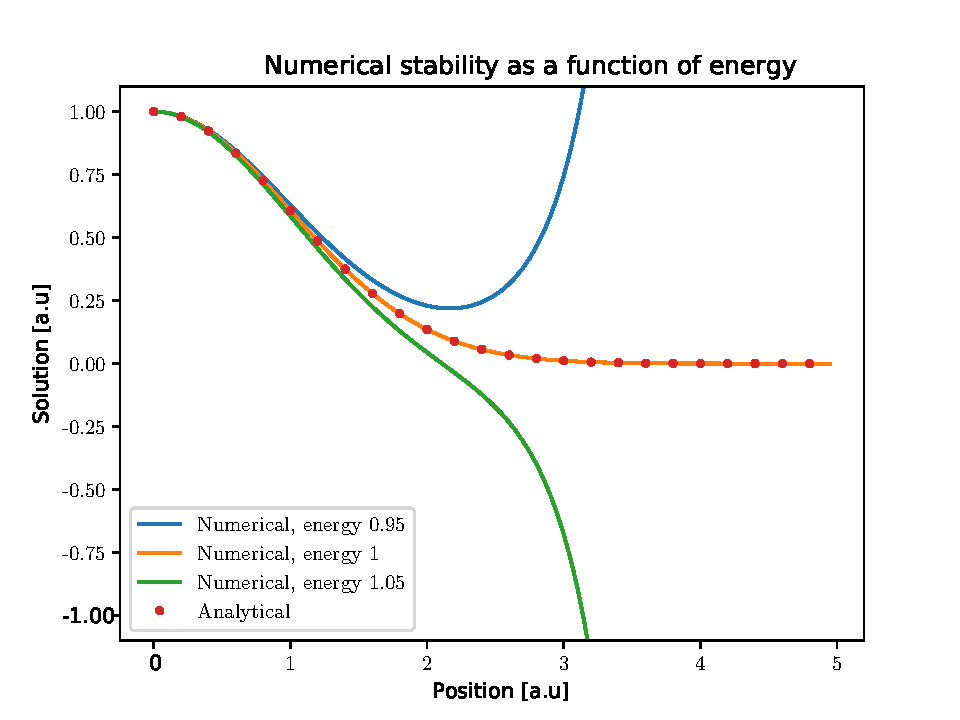
\includegraphics[width=\textwidth]{images/Quantum_oscillator-0}}
\end{minipage}
\caption{Figure \ref{fig:prec:a} presents response amplitude as a function of frequency. Figure \ref{fig:prec:b} presents the phase-shift, dashed line denotes value $3\pi/4$ (value when the phase-shift is a quater of the whole period).
Both figures show that the resonance frequency can be estimated as 136.4(1) Hz.}
\label{fig:prec}
\end{figure}


\section{References}

\begin{enumerate}
	\item C. E. Froberg, Introduction to Numerical Analysis, Addison Wesley, 1969.
	\item Joint work, Solutions of Schrodinger's equation by numerical integration, University of Oxford, 2018
	\item R. Schankar, Principles of Quantum Mechanics, Springer, 2008
\end{enumerate}

\end{document}
